\chapter{Application} % 

\section{Pump modelling}

%The objective of the model is to try to find same physical behaviour as the experimental data. We call that digital twin.

\autoref{fig:RESEDA_Model} illustrates the model of the pump on a $yz$ plane, for $x=0$. The suction pipe has a length of $H = 10 R_1$, allowing the near-wall boundary lawer to develop. Then, a cylinder, where the IBM and MRF will be applied, containing the impeller, is defined (the impeller in .stl can be find on github\footnote{\url{https://github.com/fromano88/CentrifugalPump}}).
At the entrance of the impeller/outlet of the suction pipe junction and at the outlet of the impeller/inlet of the diffuser junction, there was leakage as the whole impeller that was moving during the experiment.
We assume a zero-leakage as we aren't in a very hight mass flow rate.

In our simulation, the z-axis aligns with the rotational axis, and the reference frame is centred at the impeller. The plane at $z = 0$ divides the diffuser into two identical halves.

\begin{figure}[H]
    \centering
    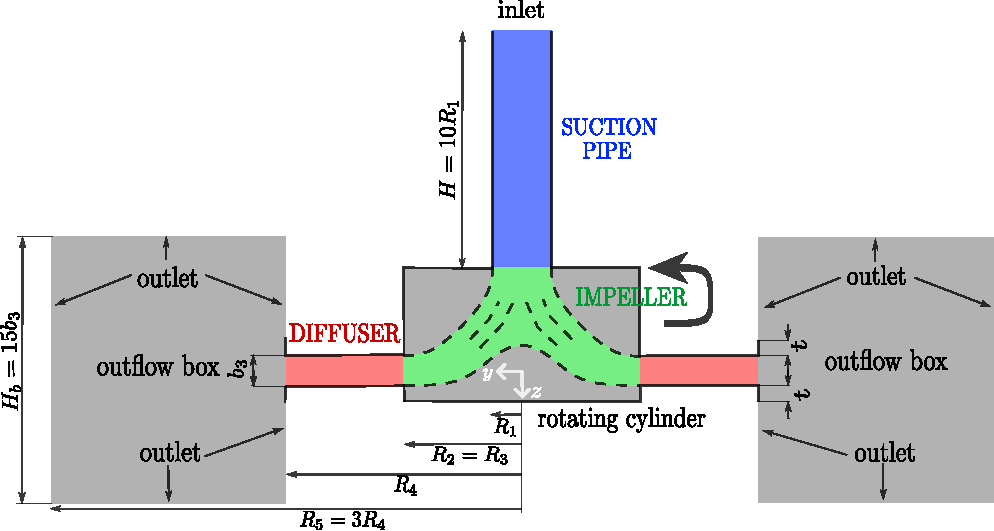
\includegraphics[width=1\textwidth]{images/model/RESEDA_sketch.pdf}
    \caption{Model of the RESEDA benchmark}
    \label{fig:RESEDA_Model}
\end{figure}

Boundary conditions are defined as follows:
\begin{itemize}
    \item[$-$] Inlet: velocity inlet
    \item[$-$] Outlet: pressure outlet
    \item[$-$] Wall: no-slip wall
\end{itemize}

To process CFD, we need to discretize the numerical model of the pump. The mesh is generated using the \texttt{blockMesh} utility, which is a built-in OpenFOAM tool. It is composed of around 11 million hexahedral cells. (quasi only, excepted some interface, cf \autoref{fig:interfaceMesh}). We don't need complex mesh because we don't need to fit the geometry of the impeller as we use IBM.

\begin{figure}[H]
    \centering
    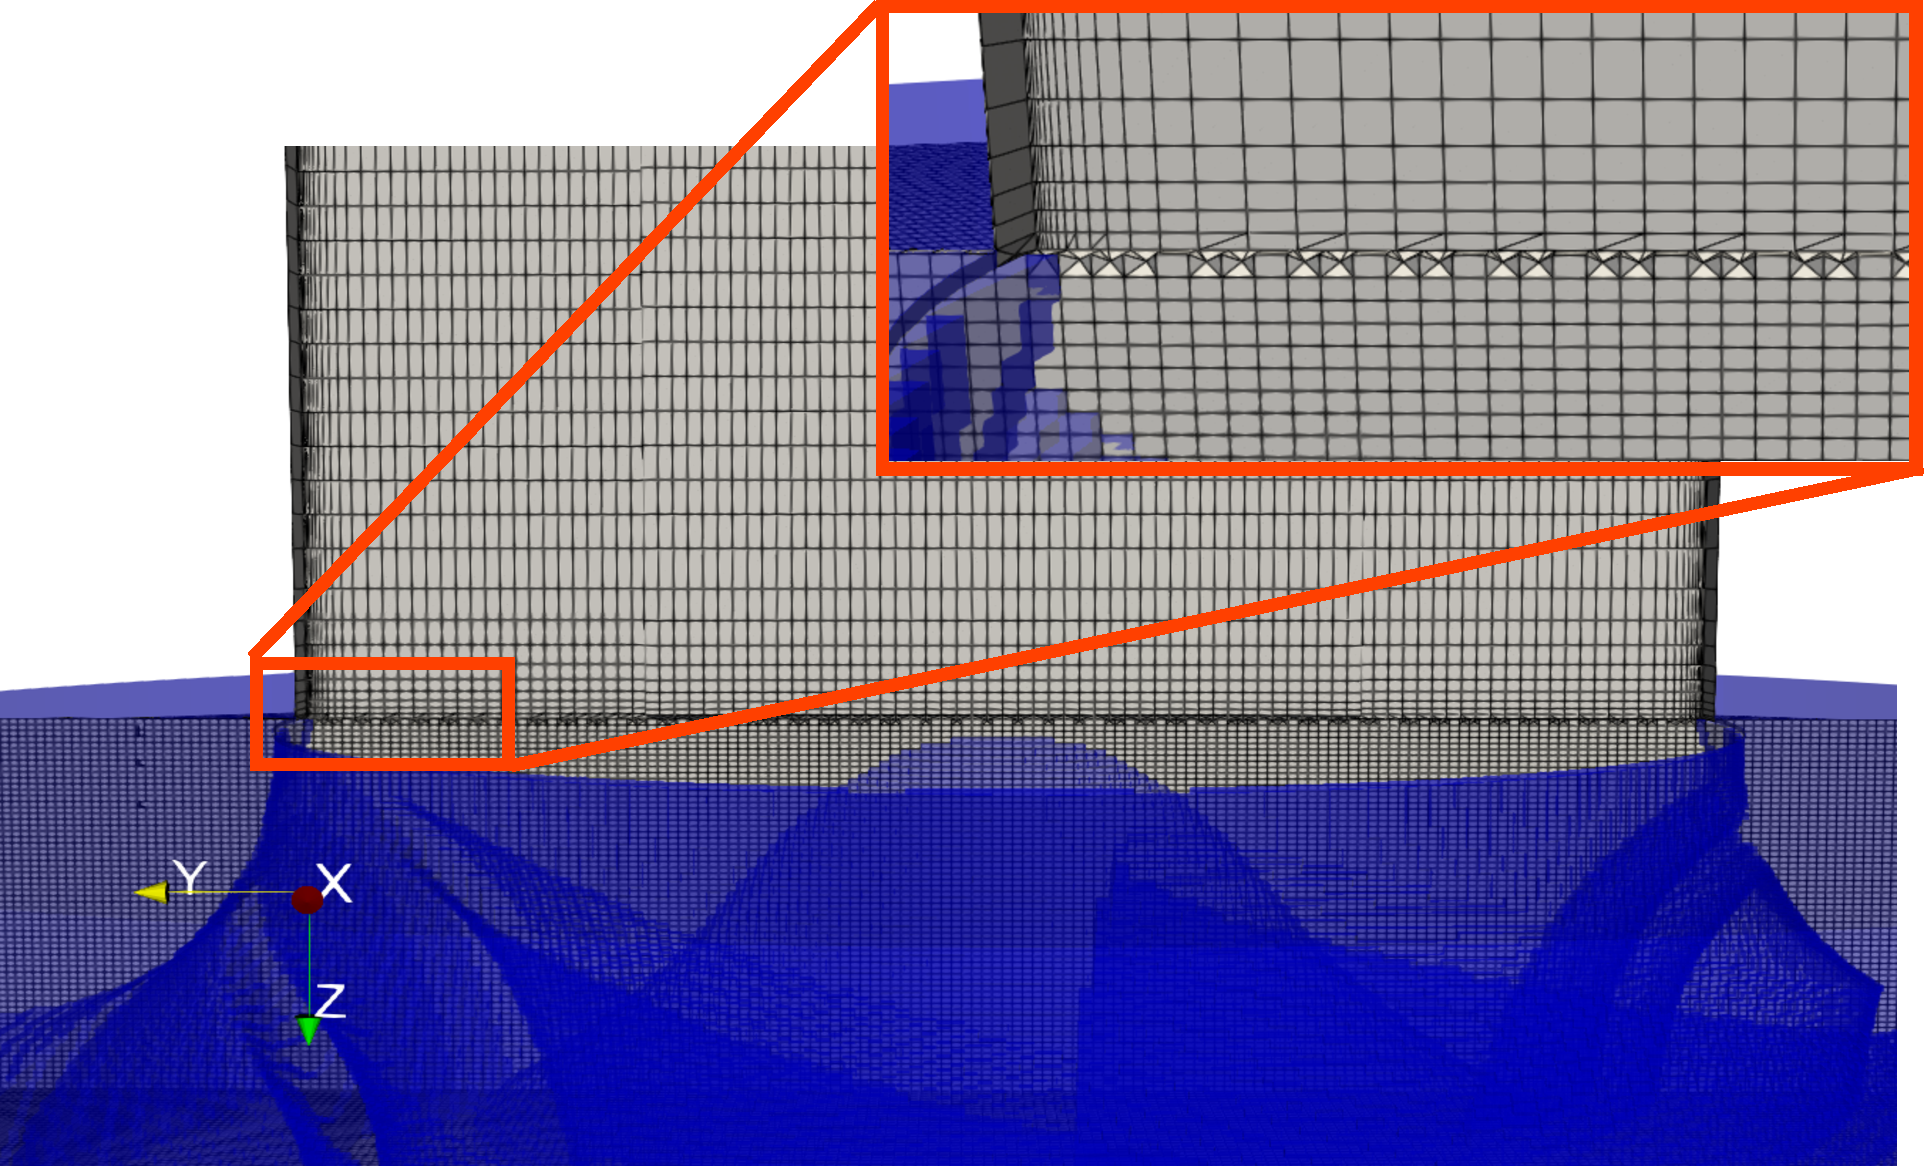
\includegraphics[width=0.5\textwidth]{images/numericalPump/frontalView.pdf}
    \caption{Mesh interface between the pipe and the impeller}
    \label{fig:interfaceMesh}
\end{figure}


Regarding the near-wall treatment, at the suction pipe, y + envegale 1, enabling direct resolution of the viscous sublayer and imposition of boundary conditions without wall functions. On the other hand, the highest y + value in the body-fitted regions corresponds to y + envegale 83, so some of the mesh elements (mainly close to the lower wall of the diffuser) are located in the logarithmic region, thus requiring wall functions. Within the rotating cylinder and around the impeller, the mesh resolution yields y + envegale 100. The friction velocity u tau is assumed to be around 20 - 25 times smaller than the peripheral velocity U2 . The
blades are discretised to ensure an average of six mesh elements across their solid thickness, preventing excessively thin regions.


The penalisation coefficients used in the \autoref{eq:IB} are defined as follows:


\begin{align}
    \boldsymbol{u}_{\text{ib}} &= \cancel{\boldsymbol{u}_r} + \boldsymbol{\Omega} \times \boldsymbol{r} \\
    \mathcal{K}_{\text{ib}} &= 0 \\
    \omega_{\text{ib}} &= \left( \omega_{\text{vis}}^2 + \omega_{\text{log}}^2 \right)^{1/2}
\end{align}

where $\boldsymbol{u}_r = 0$, $\omega_{vis}=\frac{6 \nu}{\beta_1 y_{\mathrm{ref}}^2}$ is the viscous sublayer and $\omega_{log} = \frac{\sqrt{\mathcal{K}}}{C_\mu \kappa y_\mathrm{ref}}$ is the logarithmic region (see \ref{fig:NearWallModelling}).


\newpage
\section{Experimental data and pre-processing}
\label{sec:Experimental_data_and_pre-processing}

As discussed in \autoref{sec:stateOfArt}, the RESEDA benchmark facility is located at LMFL, where PIV and pressure data have been acquired.


\begin{figure}[H]
    \centering
    \begin{subfigure}[b]{0.47\textwidth}
        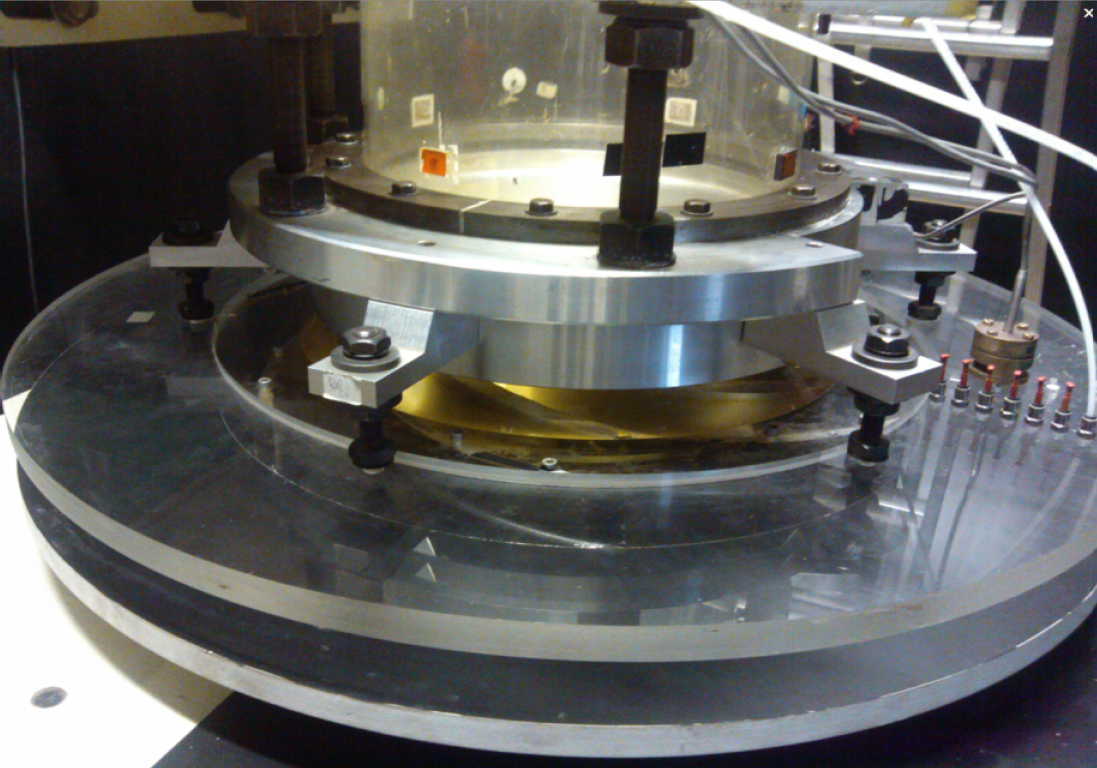
\includegraphics[width=\textwidth]{images/experimentalPump/diffuser.png}
        \caption{Vaneless diffuser of the centrifugal pump}
        \label{fig:diffuer}
    \end{subfigure}
    \hfill
    \begin{subfigure}[b]{0.46\textwidth}
        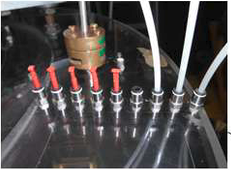
\includegraphics[width=\textwidth]{images/experimentalPump/pressure_taps.png}
        \caption{Pressure taps on the diffuser}
        \label{fig:pressureTaps}
    \end{subfigure}
    \caption{Diffuser and pressure taps of the centrifugal pump}
\end{figure}


The operating conditions of the machine were:

\begin{table}[h!]
    \centering
    \begin{tabular}{c c c}
        \multicolumn{3}{c}{\textbf{Impeller characteristics}} \\ \hline 
         $R_1$ & Tip inlet radius & $141.1\,mm$  \\
         $R_2$ & Outlet radius & $257.5\,mm$ \\ 
         $Z$ & Number of blades & $7$ \\
         $Q_d$ & Design flow rate & $0.236\,m^3/s$ \\ % 0.256 ???
         $K$ & Mean blade thickness & $9\,mm$ \\
         $\Omega$ & Rotating velocity & $1\,200\,rpm$ \\ 
         $\beta_2$ & Outside blade angle (from peripheral velocity $U=R_2\Omega$) & $22.5^{\circ}$ \\ \hline \hline
        \multicolumn{3}{c}{\textbf{Vaneless diffuser characteristics}} \\ \hline
         $b_3$ & Diffuser width & $38.5\,mm$ \\
         $R_3$ & Inlet radius (without leakage, i.e., $R_3=R_2$) & $257.5\,mm$ \\
         $R_4$ & Diffuser outlet radius & $385.5\,mm$ \\
         $t$ & Thickness of the upper and lower sections of the diffuser & $20\,mm$
    \end{tabular}
    \caption{Summary of the main geometrical and operating parameters of the impeller and diffuser at design conditions} % , employed in the numerical modelling of the centrifugal pump.
    \label{tab:pump_parameters}
\end{table}


\begin{figure}[H]
    \centering
        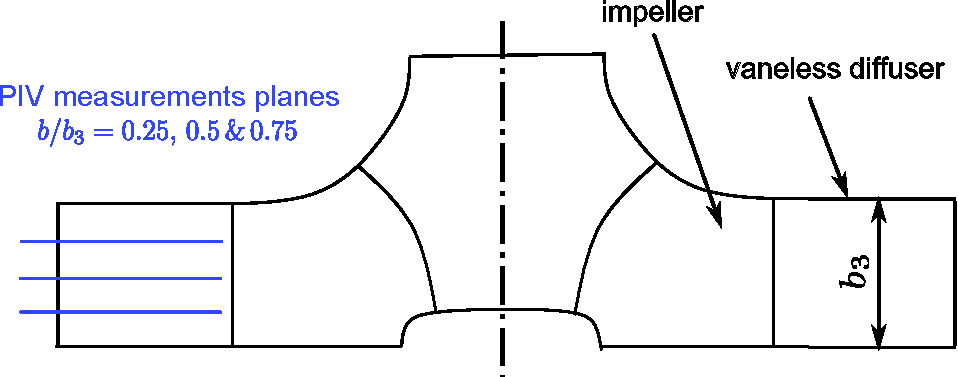
\includegraphics[width=0.6\textwidth]{images/PIV_measurements_sketch.pdf}
        \caption{Position of the PIV planes on the diffuser}
        \label{fig:PIVMeasures}
\end{figure}

\begin{figure}[H]
    \centering
        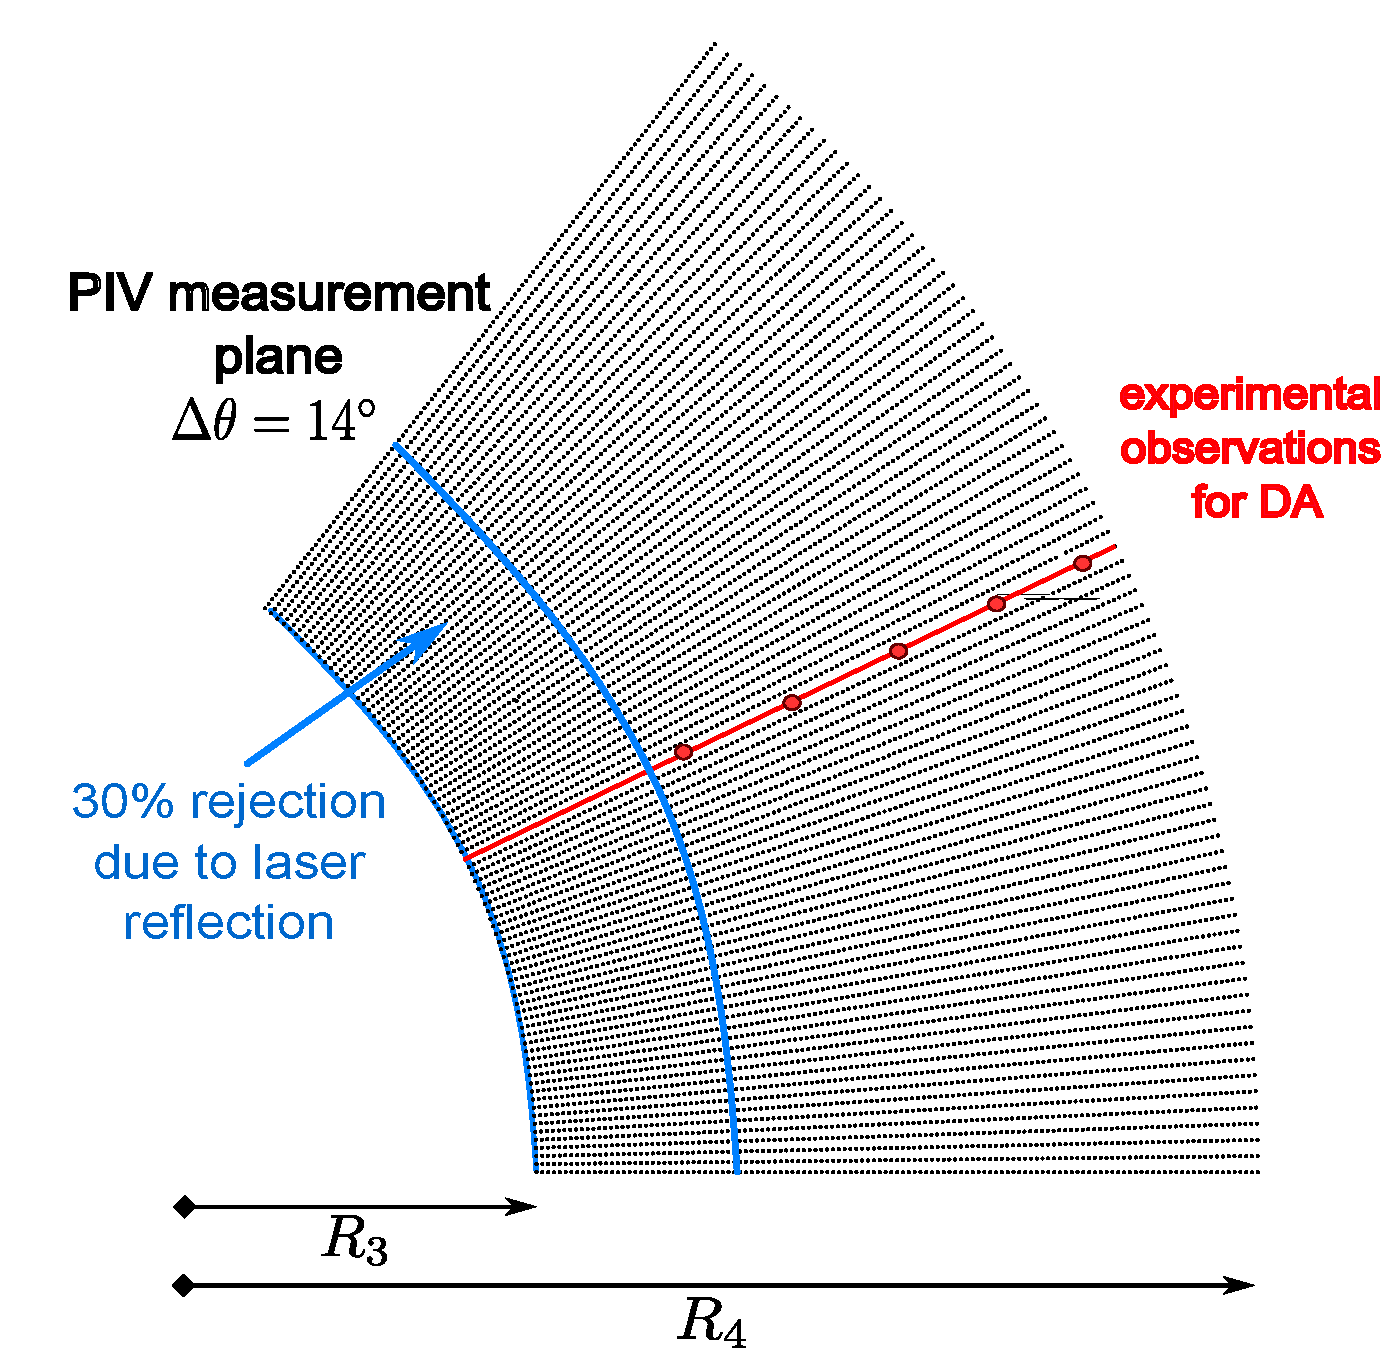
\includegraphics[width=0.5\textwidth]{images/polar_slice_avg_theta_trimmed.pdf}
        \caption{Position of the PIV points on a polar slice of the diffuser}
        \label{fig:polar_slice_avg_theta_trimmed}
\end{figure}






\paragraph{PIV data} Data is stored in a directory structure that contains six directories.
The six directories correspond to two tests realised at 25\%, 50\% et 75\% of the diffuser height.
Each test was repeated twice for the same operating condition and the same height ($R_1$, $R_2$).
In each directory, there are 1581 files corresponding to instantaneous ASCII data file.
The ten columns are corrresponding to%:

\begin{center}
    $x(m),y(m),V_x(m.s^{-1}),V_y(m.s^{-1}),r(m),\theta(rad),Vr(m.s^{-1}),V_{\theta}(m.s^{-1}),V_z(m.s^{-1}),\textit{Unknown}$
\end{center}

And the 10,125 lines correspond to the 81 locations over x and 125 locations over y of the PIV.
The PIV data is acquired in a rectangular zone of 0.08 m x 0.124 m.
The cathesian coordinates are given in a local system, where the absolute origin is at the center of the pump.


\begin{figure}[H]
    \begin{center}
        \begin{tikzpicture}
            \begin{axis}[
                axis equal,
                xlabel={$x$ (m)},
                ylabel={$y$ (m)},
                width=8cm,
                height=12cm,
                grid=both,
                xmin=0, xmax=0.08,
                ymin=0, ymax=0.124,
                %title={PIV acquisition zone}
            ]
            \draw[red, very thick, dashed] (0.0245, 0) -- (0.0245, 0.124);
            \node[red, rotate=90] at (0.053-0.031, 0.062) {$\theta = x_{abs} = 0$};


            % CentreAbs: (0,0)    -> CentreRel: (-0.0245,0.257.5)
            % BoutRel: (0.06, 0.12) -> boutAbs: ...

            \draw[darkblue, very thick, dashed] (0.037756, 0) -- (0.0445, 0.124);
            \draw[darkblue, very thick, dashed] (0.051012, 0) -- (0.0645, 0.124);
            %\draw[darkblue, very thick, dashed] (0.02*(0.2575/0.3855)+0.0245, 0) -- (0.0245+0.02, 0.124);
            %\node[darkblue, rotate=90] at (0.053-0.031, 0.062) {$\theta = x_{abs} = 0$};
            
            \draw[->, >=stealth, color=darkblue, thick] (0.0245, 0.0145) -- (0.07-0.031, 0.0145);
            \node[darkblue, rotate=0] at (0.062-0.031, 0.017) {$\vec{x}$}; % _{abs}

            \draw[->, >=stealth, color=darkblue, thick]  (0.0245, 0.0145) -- (0.0245, 2*0.0145);
            \node[darkblue, rotate=0] at (0.021, 0.0195) {$\vec{y}$}; %_{abs}

            \draw[->, >=stealth, color=red, thick]  (0.0245, 0.1) -- (0.0245, 0.1145);
            \node[red, rotate=0] at (0.062-0.032, 0.108) {$\vec{U_{r}}$};

            \draw[->, >=stealth, color=red, thick]  (0.0245, 0.1) -- (0.01, 0.1);
            \node[red, rotate=0] at (0.0245-0.01, 0.1-0.005) {$\vec{U_{\theta}}$};


            \addplot+[
                only marks,
                mark=*,
                mark size=0.3pt,
                color=blue
            ] table [x index=0, y index=1] {autre/points_piv_tikz.txt};
            \end{axis}
        \end{tikzpicture}
    \end{center}
    \caption{PIV acquisition zone in the RESEDA experiment, with orientation of the $(r,\theta)$ velocity components.}
\end{figure}

\textbf{Pre-processing on the velocity data}\footnote{
In the numerical simulation, the z-axis is toward the center of the Earth, unlike in the experiment, where it is upwards.
Then, the wheel rotates counterclockwise in the numerical simulation frame and counterclockwise in the experiment.
Here, the numerical simulation formalism was the reference for the frame.
}

In this work, we aim to improve the numerical model of a centrifugal pump using experimental data obtained from PIV. On one side, we have a numerical simulation of the pump (the digital twin), and on the other side, experimental PIV measurements. To combine the strengths of both, we use data assimilation, a method that updates a numerical model using real-world data.
We specifically use the EnKF, a data assimilation technique that relies on an ensemble of simulations to estimate and reduce uncertainty in the model. The process can be summarized in two main steps:

\begin{enumerate}
    \item \textbf{Forecast Step} We run a steady-state numerical simulation of the pump using the Multiple Reference Frame (MRF) and the IBM methods. This yields an ensemble of model states, representing the expected flow field within the pump.
    \item \textbf{Analysis Step} We compare the simulation results with the experimental PIV data. To do this, we interpolate the PIV measurements onto the mesh of the numerical model, creating an ensemble of observation vectors. We then compute the difference between the simulated and measured data, known as the innovation (see mathematical formulation in \autoref{subsec:CFD_governing_equations}). This innovation is used to update the ensemble through the EnKF algorithm, improving the numerical model.
\end{enumerate}

\newpage

The measurements are done as follow:

\begin{enumerate}
    \item \textbf{Nature of the Numerical Simulation} The simulation is stationary (time-independent) and uses the MRF approach to model rotation. While the velocity field remains constant over time, it varies in space, especially in the diffuser region. Because of the pump's geometry, we expect a periodic velocity pattern that repeats every 1/7th of a revolution (due to the 7 blades). However, this repeating pattern is not clearly visible in unsteady simulations due to wake deformation.
    \item \textbf{Nature of the Experimental Data} The PIV system captures 49 images per full rotor revolution, meaning there are 7 images between two successive blades. In the rotating frame of reference, each image corresponds to a phase shift of approximately 360°/49.
\end{enumerate}


Ideally, to compare consistent datasets, we could run a time-resolved unsteady simulation and synchronize it with the PIV snapshots. However, for this initial study, we chose to work with a steady MRF simulation.
%Although we could attempt to reconstruct the spatial velocity field from the phase-averaged PIV data (as done by Dazin et al. \cite{dazinHighspeedStereoscopicPIV2011a}), there are two main limitations:

To address these issues, we opted to average the PIV data over time, which is equivalent to spatial (azimuthal) averaging in the rotating frame. On the simulation side, we therefore perform azimuthal averaging of the numerical results to make them consistent with the experimental data.
This approach ensures that the data fed into the EnKF, both the forecast and the observations, are comparable and compatible in both spatial and statistical sense.

\subparagraph{1.}

First, we need to determine how to convert the coordinates from the local system to the absolute system.
We observe that between lines 55 and 56, the radius remains constant while the angular position \(\theta\) shifts from below \(\pi\) to values above \(\pi\). 
For the 75\% plane, a similar approach is used, but between lines 65 and 66, due to experimental constraints.

We also plotted \(x\) versus \(\theta\) for three different values of \(\theta\) and found an intersection point at \(x = 0.0245\).
Therefore, we now know that for \(x = 0.0245\), \(\theta = \frac{\pi}{2}\).

The absolute coordinate system is then defined by the following equations:
\begin{equation}
    \begin{cases}
        x_{\text{rel}} = x_{\text{abs}} + 0.0245 \\
        y_{\text{rel}} = x_{\text{abs}} + R_{2} \\
    \end{cases}
\end{equation}

with $R_{2} = 257.5$ mm

\subparagraph{2. Average}

Since we are dealing with a stationary simulation (time-invariant), we perform a time average of the data.
There are approximately 49 velocity maps (i.e., 49 files) per impeller rotation. To compute the time-averaged field, we average over the azimuthal angle \(\theta\).%, which spans from 0 to approximately 211 radians. This corresponds to the 49 snapshots.
These files are distributed across six directories, each corresponding to a different acquisition plane.


\subparagraph{3. Sampling}

We further average the data between radii \(R_1\) and \(R_2\), resulting in three files of size $81 \times 125$ lines and $10$ columns.
At this stage, we retain only the data along the line \(x = 0.0245\). More precisely, we average the data between \(x = 0.024\) and \(x = 0.025\).
Finally, the data are truncated at line 89, where the radius exceeds 0.3~m. This truncation is necessary due to laser reflections on the pump casing during the PIV experiments.\footnote{Concretely, to average the data over the angle \(\theta\), we modify the interpolation function in CONES.
Instead of read coords, the interpolation function read the data in a file named \texttt{coords\_seventh.txt}.
Then, it computes the interpolation and average the data over the angle \(\theta\) (between -$\pi/7$ and $\pi/7$), by doing a sum over \(\theta\) and dividing by the number of points (150). To go back from 150x5x3x3 (to detail) to 5x3x3 data. All of those computations are made in a cylindrical referencial.}


\subparagraph{4.Shaping for CONES}
CONES keeps data in a particular way. We need to convert the data in a format that CONES can read.
From 3 files (of $10 \times 81 \times 125$ elements) to the files 
\texttt{fieldCylindrical.txt} (of size $n_{\text{obs}} \times n_{\text{dim}} \times n_{\text{vars}}$ lines) 
and \texttt{obs\_coordinates.txt} (of size $n_{\text{obs}}$ lines and $n_{\text{dim}}$ columns).

\subparagraph{5.Creation of a file for the interpolation}

Finally, we need to create the \texttt{coords\_seventh.txt} file for the interpolation function in CONES.
We don't just use the coordinates of the points in the PIV data, beacause we want to average over the angle \(\theta\) on the pump. The numerical simulation is $2\pi/7$ periodic, so we interpolate in 150 points over theta between 0 and $2\pi/7$, as illustrated in the \autoref{fig:diffuserMesh}. %$\frac{2\pi}{7}$
To do that, we just take the \texttt{obs\_coordinates.txt} file and duplicate 150 times the points over the angle \(\theta\) (between $-\pi/7$ and $\pi/7$). In our case, we chose 150 that will aproximately correspond to the shap of a cell at this radius.
To be consistent with axis further, we take points between $-\pi/7 + \pi/2$ and $\pi/7 + \pi/2$.
\footnote{Concretely, to average the data over the angle \(\theta\), we modify the interpolation function in CONES.
Instead of read coords, the interpolation function read the data in a file named \texttt{coords\_seventh.txt}.
Then, it computes the interpolation and average the data over the angle \(\theta\) (between -$\pi/7$ and $\pi/7$), by doing a sum over \(\theta\) and dividing by the number of points (150). To go back from 150x5x3x3 (to detail) to 5x3x3 data. All of those computations are made in a cylindrical referencial.}

\begin{figure}[H]
    \centering
    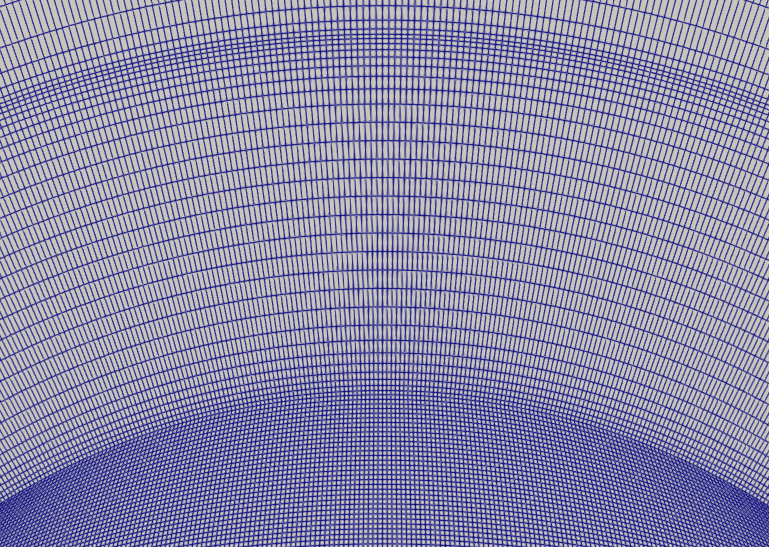
\includegraphics[width=0.4\textwidth]{images/numericalPump/diffuseurMesh.png}
    \caption{Imaginary points to compute the average of the data over the angle \(\theta\) in the diffuser}
    \label{fig:diffuserMesh}
\end{figure}

\begin{figure}[H]
    \centering
    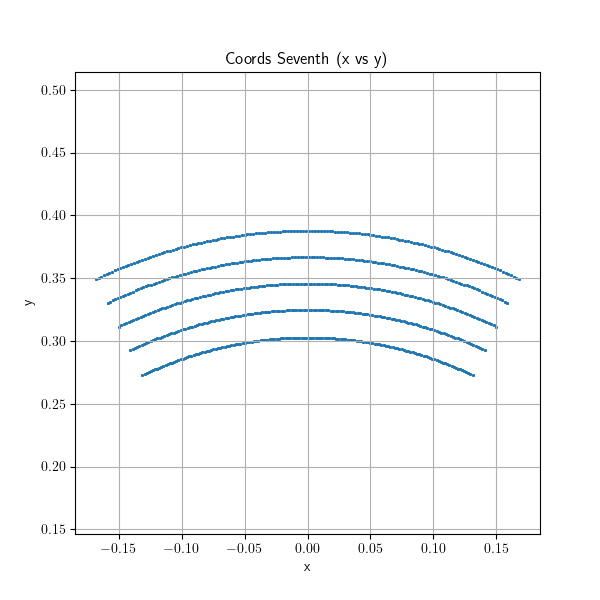
\includegraphics[width=0.5\textwidth]{images/coordsSeventh.png}
    \caption{Interpolation points over 360/7 degrees}
    \label{coordsSeventh}
\end{figure}

\paragraph{Pressure data}

In addition to the nine pressure tapes on the diffuser, Dazin et al.~\cite{dazinHighspeedStereoscopicPIV2011a} have also captured (\autoref{fig:PumpPerf}) the inlet and outlet pressure that allows to compute the global performance of the pump, that matches with M. Fan simulation \cite{fanEffectLeakagePerformanceb}% (eq to approximately \(\eta\) = 0.4).

\begin{figure}[H]
    \centering
    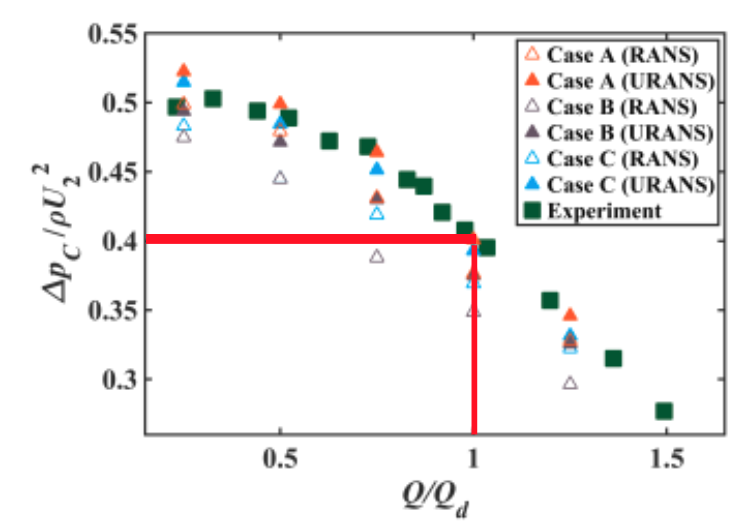
\includegraphics[width=0.65\textwidth]{images/experimentalPump/perfo2.png}
    \caption{Overall pump performance versus reduced pump flow rate Q\cite{dazinHighspeedStereoscopicPIV2011a}}
    \label{fig:PumpPerf}
\end{figure}

As we are at $Q/Q_d = 1$, we can retreive:

\begin{equation}
    \frac{\Delta P_{P}}{\rho U_{2}^{2}} = \eta \Leftrightarrow \Delta P_{P} = \rho U_{2}^{2} \eta
\end{equation}

For the high-fidelity value, we can find experimental data from the same pump \cite{fanEffectLeakagePerformanceb}, that's matches with M. Fan simulation (eq to approximately \(\eta\) = 0.4). So we can also compute:

${U_{2}}$ is the impeller tip speed computed from the impeller diameter and the rotation speed of the pump.

\begin{equation}
    U_{2} = {(\Omega \times R2)}^2 = {(2 \times \pi \times \frac{1200}{60} \times 0.2566)}^2 = 32,2 m/s
\end{equation}

Finally:

\begin{equation}
    \Delta P_{p} = 1.225 \times 32.24^2 \times 0.4 \approx 415~\text{Pa}
\end{equation}



%As we are in a steady simulation, the restult of the numerical pressure is divided by the density of the fluid.

%\begin{equation}
%    \Delta P_{P} = 32.2^{2} \times 0.4 = 415 Pa
%\end{equation}




\newpage
\section{IBM preliminary results}%and modifications on OpenFOAM 
\label{sec:IBM_preliminary_results}

%\textbf{IBM preliminary results}

Once the pump model is implemented in OpenFOAM, we can run the simulation with the IBM.
After empirical tests and with experience of the laboratory, we found that the parameters $\mathbf{D} = (3e7, 3e7, 3e7), D_k = 3e7$ and $D_{\omega} = 3e7$ are a good starting point for the IBM parameters. And it verifies a converged CFD solution.

\begin{figure}[H]
    \centering
    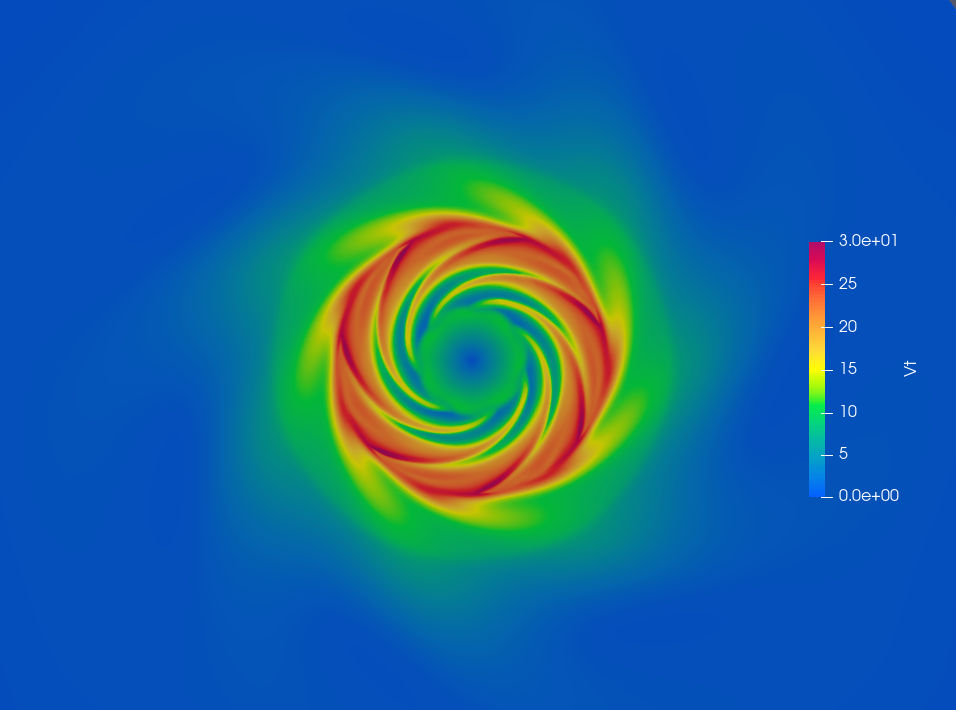
\includegraphics[width=0.65\textwidth]{images/numericalPump/mvt.png}
    \caption{First results of the IBM for all parameters equal to 3e7. Slice at $z=0$ for $\mathbf{D} = (3e7, 3e7, 3e7), D_k = 3e7, D_{\omega} = 3e7$}
    \label{fig:Pumpfirst}
\end{figure}

With the conditions specified in the \autoref{tab:pump_parameters}, and a value of 3e7 for the all five forcing parameters, we obtain these velocity profils comparing the velocities of the simulation and of the PIV data. Both are averages over time and over the angle \(\theta\):

\begin{figure}[H]
    \centering
    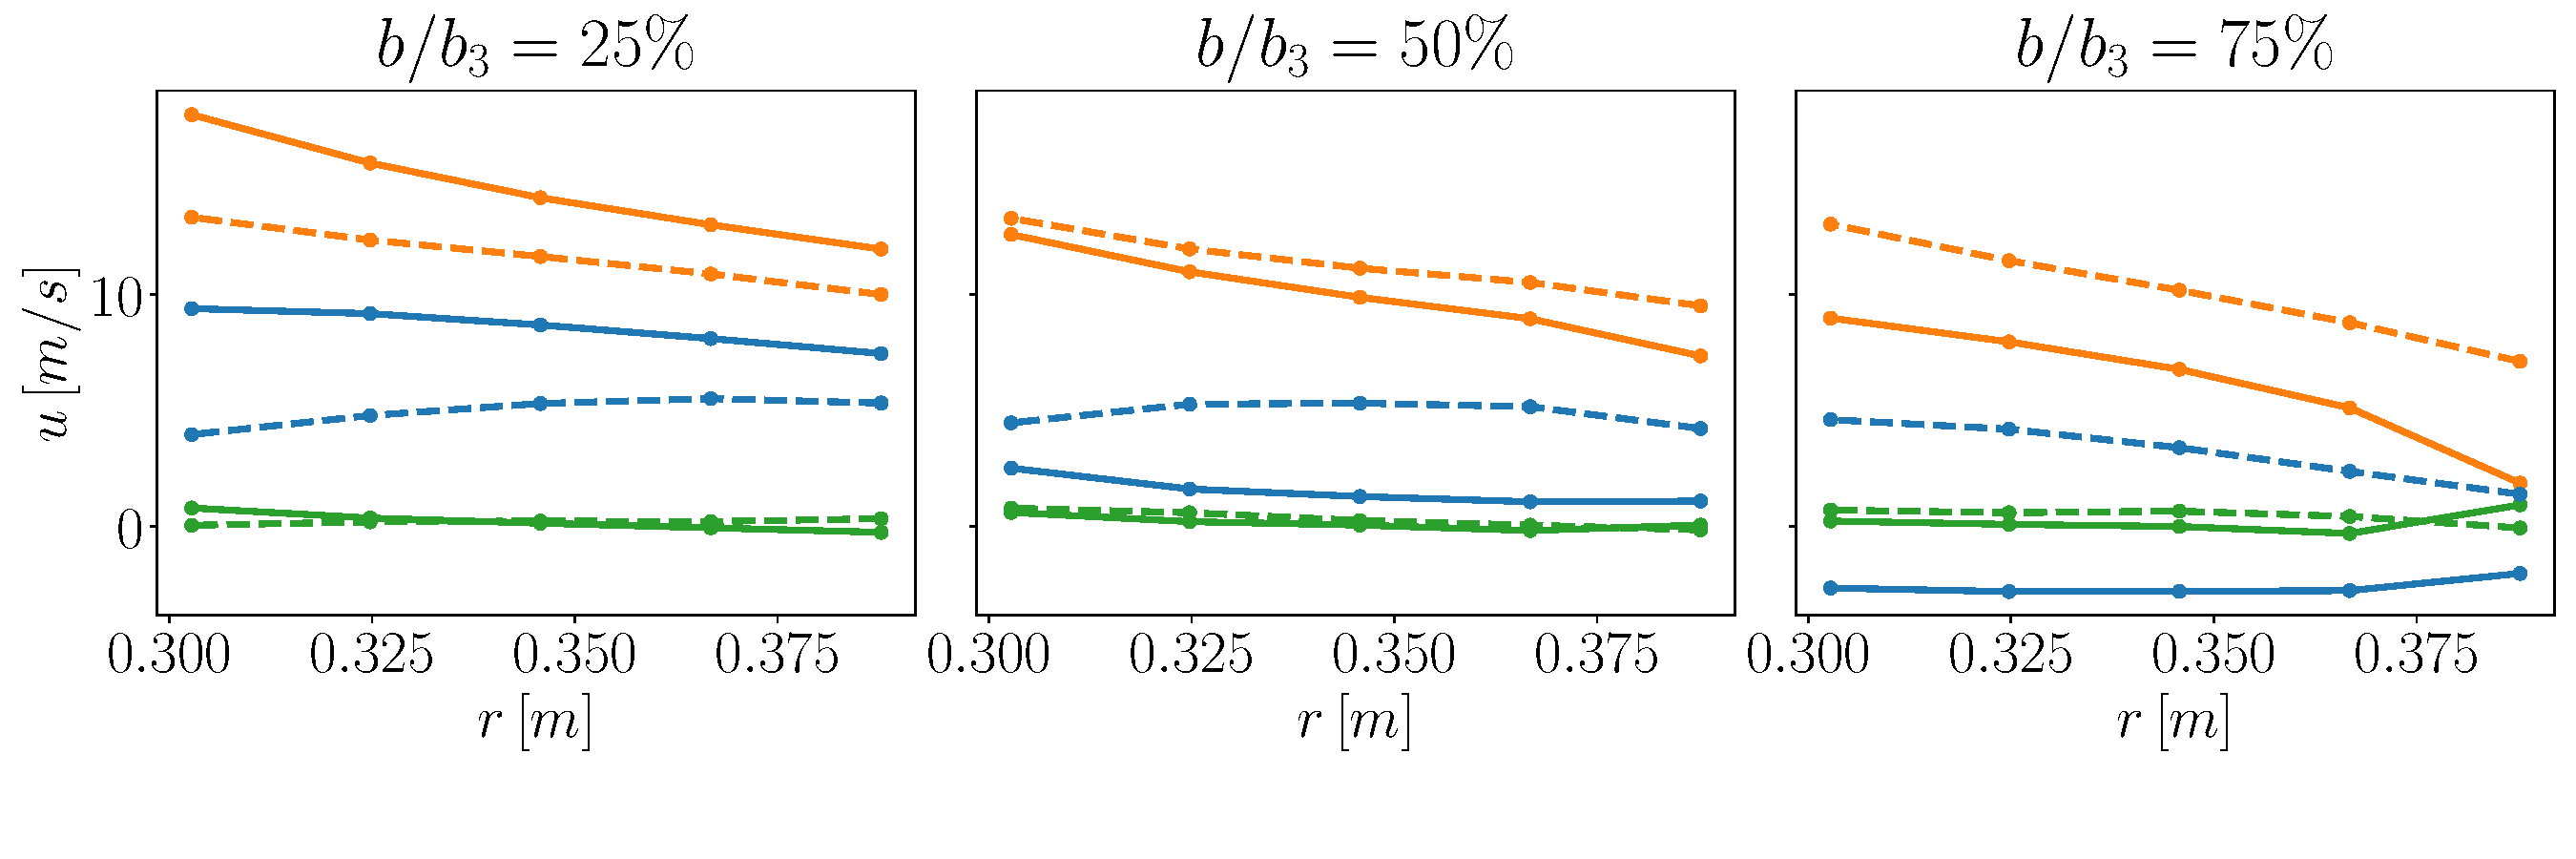
\includegraphics[width=1\textwidth]{images/numVSxp.pdf}
    \caption{Comparison between the profiles inside the diffuser for the numerical simulation (continuous lines), and the PIV data (dashed lines). In particular, (\protect\bluelinePython) represents the radial velocity $u_r$, (\protect\orangeline) depicts the azimuthal velocity $u_\theta$, and (\protect\greenline) illustrates the vertical velocity $u_z$. $\mathbf{D} = (3e7, 3e7, 3e7), D_k = 3e7, D_{\omega} = 3e7$} % \textit{(a)} Position of the PIV measurement planes, \textit{(b)} simplification of the experimental data (time- and azimuthally-averaged) for employment in the Data Assimilation experiment, and \textit{(c)} c
    \label{fig:numVSxp}
\end{figure}

As seen in \autoref{fig:polar_slice_avg_theta_trimmed}, we use five observation points on the three PIV plans.
Our goal is to make these curves fit as much as possible.


We have already seen that there is a notable difference beteween the experimental and numerical radial velocity in the plan at 75\%. The numerical simulation predicts a negative velocity instead of a positive one. This is explained by a non physical recirculation bubble as you can see in the \autoref{fig:LIC} deeper exmplained in the following part. %\autoref{...}

A good indicator of the accuracy of the simulation is the performance of the pump. It's directly linked to the pressure difference between the outlet and the inlet. As seen in the previous \autoref{sec:Experimental_data_and_pre-processing}, we should obtain around 415Pa. In our case, we obtain a pressure difference of around 306 Pa, far from what we expect.



%At pump flow rate = pump design flow rate So Q?/Q? =1
%\subsection{Modifications on OpenFOAM} %Preparation   %  and CONES for the DA

%S'aider du plan de la présentation MALEAF + thèse M
%Expliquer comment j'applique la DA sur le cas test de la pompe centrifuge (pas d'equation)


\section{First simple application of the DA}
\label{sec:Application_of_the_DA}

As represented on the \autoref{fig:CONES}, we need to adapt the OpenFOAM and CONES codes to apply the EnKF on the centrifugal pump case. Among others, the MPI exchanges are coded.

\textbf{Modifications on OpenFOAM}
Previously, OpenFOAM has been adapted to our case, including the implementation of the IBM and MRF methods, as well as the definition of the mesh and boundary conditions. Now, we need to adapt OpenFOAM to work with CONES, by including MPI processes that will allow to run a simulation with variable IBM parameters and that will be able to return interpolated averaged velocities to CONES.

\textbf{Adaptations on CONES}
Although CONES is already adapted to work with OpenFOAM, we still need to adjust the code to fit our specific observations.

\textbf{Test case}
Finally, we have to initialize a repesitory for the test case, i.e., the centrifugal pump. This includes defining the initial parameters, the observation points, and the initial state of the ensemble members, including a \texttt{conesDict}.


\textbf{Parameters} To determine the variance for the initial perturbation, two perspectives were considered. The experience at lab shows that an initial perturbation of around $5\%$ of variance is good. From our side, the target was that, around only one ensemble member differs by maximum approximately $1 \times 10^7$ from the previous time step, for parameter values of order $3 \times 10^7$. With 30 ensemble members, this corresponds to about $95\%$ of the values (i.e., within $2\sigma$) being contained in the interval 
\[
[3 \times 10^7 \pm 1 \times 10^7].
\]
This leads to a standard deviation of 
\[
\sigma = 0.5 \times 10^7,
\]
or about $17\%$.
We finally choose a variance of 5\% for the first test.

Let us introduce the observation window.  
The observation window was defined by observing the number of iterations required for the influence of the IBM forcing to reach the diffuser and take the form of the converged result. Turbulence parameters were not considered for defining this window, since their effect is present throughout the domain and their influence is almost immediate (although their convergence is slower).  

The number of iterations between two analysis phases was determined by monitoring how many iterations are required for a parameter perturbation (e.g., $34\%$ change) to significantly affect the solution in the diffuser. What matters here is not full convergence, but that the solution starts to follow the correct trend. For turbulence parameters, this timescale is expected to be much shorter, since the forcing is applied everywhere in the domain.  
We determined a number of 800 iterations for the observation window.

The \texttt{conesDict} and the \texttt{controlDict} contains the parameters of the EnKF algorithm, such as the observation window and the following. In our case, we set the number of ensemble members to 30, no inflation, no state optimisation (only parameters), and an absolute observation noise on the velocity of $0.2 \, \text{m/s}$ (equivalent to $1.5\%$ of the maximum observed velocity). These parameters must be adjusted depending on the specific requirements of the simulation and the characteristics of the data. The number of iterations (800) was determined by testing the convergence trend of a single OpenFOAM simulation when parameters are modified by 34\% (i.e., seven times the standard deviation of the initial parameter perturbation). Since the standard deviation may temporarily increase with iterations, care must be taken when choosing this number.
An extract of the \texttt{conesDict} is given in appendix~\ref{annex:conesDict}.  

%MThe \texttt{conesDict} contains the parameters of the EnKF algorithm such as the following. In our case, we set the number of ensemble members to 30, an observation window of 800 iterations, no inflation, no state optimisation (only parameters), and the absolute observation noise on the velocity of $0.2m/s$ (equivalent to $1.5\%$ of the maximal observation on the velocity). These parameters have to be adjusted based on the specific requirements of the simulation and the characteristics of the data.
%The number of iterations is set to 800 by testing the tendancy of the convergence of one OpenFOAM simulation when parameters are modify of 40\%, which is 20 times the standard deviation of the initial perturbation on parameters (the standard deviation can momenta,ly increase with iterations, so we need to be careful with the number of iterations).

%As initial parameters to optimise, we use the same as in the previous section, i.e., $\mathbf{D} = (3e7, 3e7, 3e7), D_k = 3e7$ and $D_{\omega} = 3e7$, with a gaussian perturbation of 2\%.
%Comment calculer la variance que je veux mettre ?
%Expérience: 5\%
%De mon coté: je vise qu'en moyenne un membre d'ensemble ait un écart de 1e7 par rapport au temps précédent (pour des valeurs autour de 5e7), donc, pour 30 membres d'ensemble, environ 95\% = 2 sigma dans 5e7+-1e7, càd sigma = 0.5e7 = 10\%. Ensuite, le nombre d'itération entre les phases d'analyse est déterminé en regardans combien d'itération sont nécessaires pour faire varier la solution dans le diffuser (influe, rapidement, converge doucement mais ce qui nous intéresse c'est que ça prenne la tendace) lorsqu'un paramètre de forcage est modifié (supposé très inférieure pour la turbulence car appliquée de partout)


\textbf{First results}

After letting the simulation run for around 50 iterations, we obtain the first results of the optimisation with CONES. The parameters are optimised to fit the PIV data, and the velocity field is represented on a slice at $z=0$. The resulting parameters are the following: $\mathbf{D} = (4e7, 2e7, 4e7), D_k = 3e7$ and $D_{\omega} = -3e7$. The sum of the NRMSEs on the velocity field decreased, of around 20\%. The global performance of the pump didn't change significantly.
Usually, around 200 iterations are needed to converge but is not need for a first result and cost a lot of CPU time (1270 CPU $\times$ hours per EnKF iteration).


\begin{figure}[H]
    \centering
    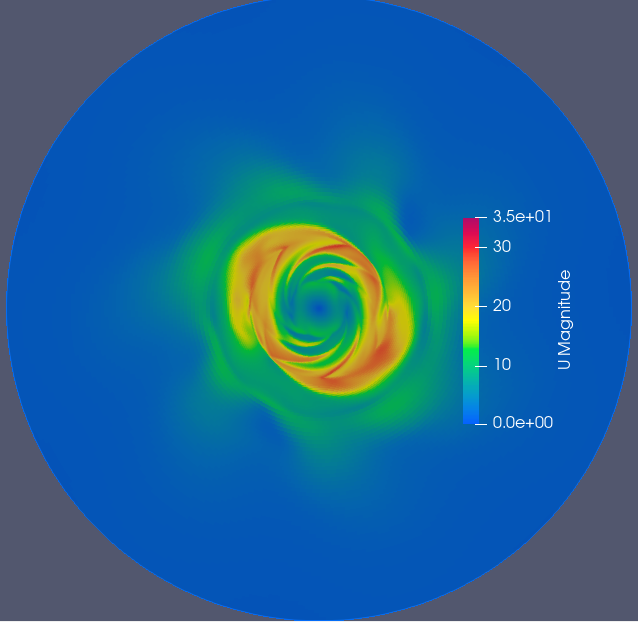
\includegraphics[width=0.65\textwidth]{images/numericalPump/assymetrie.png}
    \caption{First results of CONES optimisation. Slice at $z=0$, with $\mathbf{D} = (4e7, 2e7, 4e7), D_k = 3e7$ and $D_{\omega} = -3e7$}
    \label{fig:PumpfirstAssymetry}
\end{figure}

We would expected $D_x = D_y$ because the geometry is symmetrical, but we see that the optimisation converges to a solution where $D_x \neq D_y$. The local minimum found by the optimisation gives us a unsatisfactory solution.
$D_{\omega}$ is negative, which does not correspond to physical results.


\newpage
\section{Analysis and Results}
\label{sec:Results}

Looking at the physics of the pump CFD optimise by DA more in detail, we realize that the IBM method as applied here does not give us a physical result at all and the DA does not allow us to improve this result. It let the flow passing through the external part of the impeller (see \autoref{fig:LIC}), which is not physical. This imply a recirculation bubble in the diffuser that we would like to avoid.

\begin{figure}[H]
    \centering
    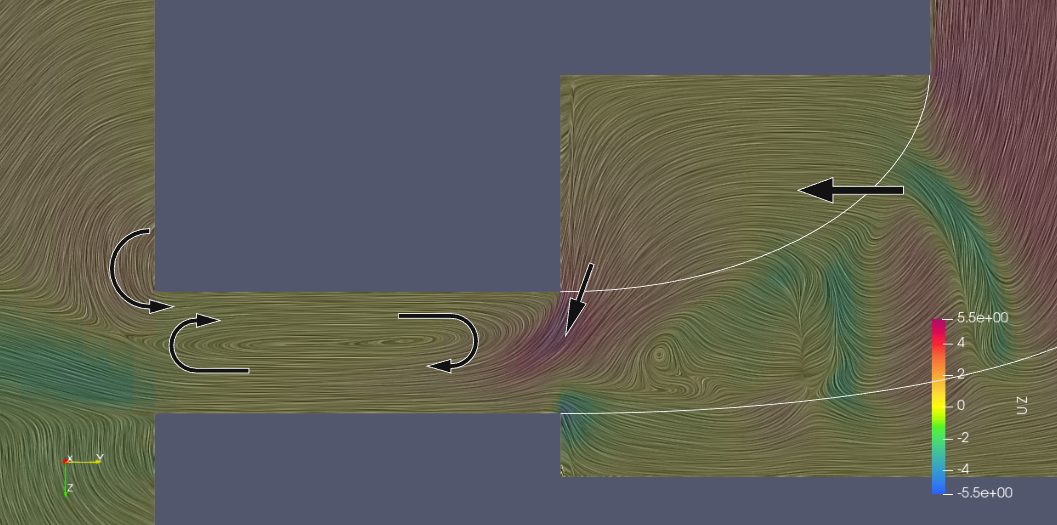
\includegraphics[width=0.8\textwidth]{images/numericalPump/LIC.png}
    \caption{Formation of the recirculation bubble in the diffuser}
    \label{fig:LIC}
\end{figure}

To try to counter this problem, a few strategies are deployed, tested separately or in combination (each DA analysis cost a lot of CPU time, so we are limited in the number of analysis we can do):

\textbf{1. $D_x = D_y$} strategy is to force $D_x = D_y$ (it helps the convergence by the way, by reducing the number of parameters to optimise).
In that case, the parameters vector is reduced to $\mathbf{D} = (D_x, D_z, D_k, D_{\omega})$.

\textbf{2. $D_{\omega} > 0$} strategy is to force $D_{\omega} > 0$, keeping a variance between each other to allow the parameters to vary.

\textbf{3. Radial expansion} strategy is to use a radial expansion of the five forcing coefficients as illustrated in the \autoref{fig:radialExpension}.
We used a second order polynomial to represent the radial expansion of the forcing coefficients, for a few raisons:
\begin{itemize}
    \item it allows to have a more complete representation of the forcing coefficients, which can help to better fit the experimental data;
    \item it allows to have a smooth variation of the coefficients over the impeller radius, which is more realistic than a constant value;
    \item it allows to describe pretty well the geometry in a quadratic way, which is more complete than a sinusoidal representation (see \autoref{fig:bladeInterpolation}) which would also require 3 parameters;
    \item three parameters are not too many so that the optimisation is not too long and the convergence is not too difficult;
    \item it permits to eliminates a step of the value to 0 at the blade tips for a continuity of order 0, which can be important for the numerical stability of the simulation.
\end{itemize}
In that case, the parameters vector change from five values to fifteen values.

\begin{figure}[H]
    \centering
    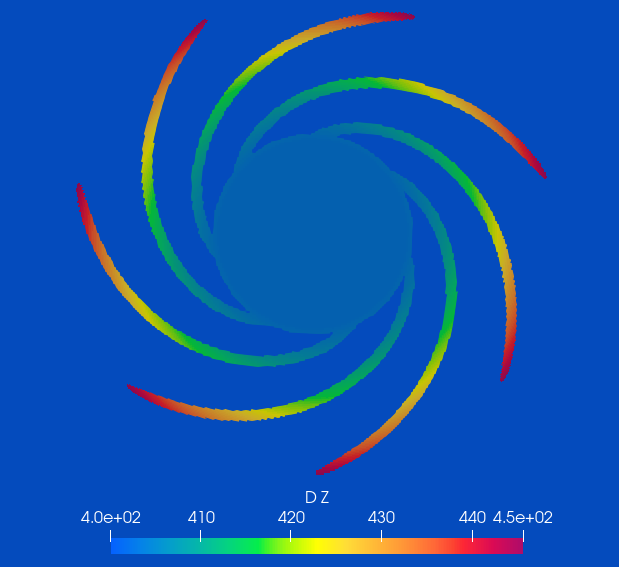
\includegraphics[width=0.5\textwidth]{images/numericalPump/radialExpension.png}
    \caption{Radial expension of Dz over the impeller radius}
    \label{fig:radialExpension}
\end{figure}

\begin{figure}[H]
    \centering
    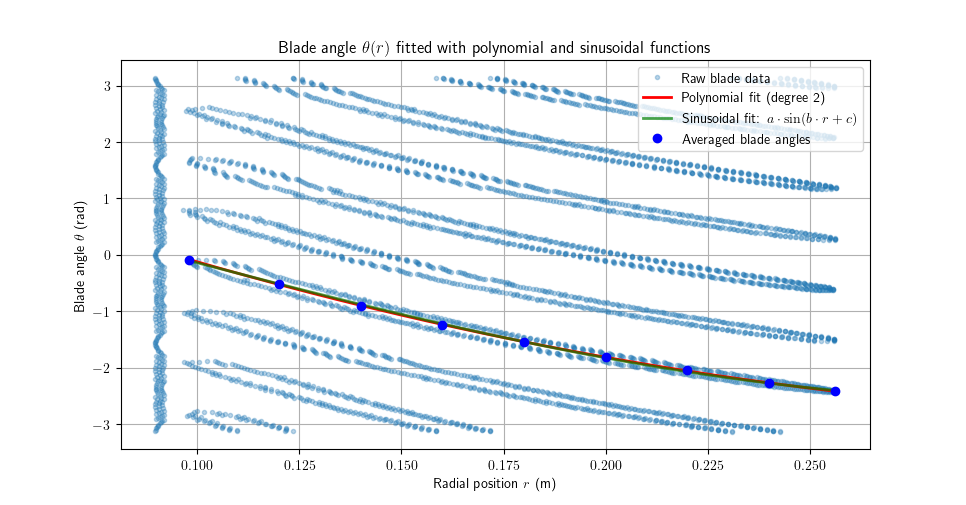
\includegraphics[width=1\textwidth]{images/blade_interpolation_1.png}
    \caption{Polynomial and sinusoidal interpolation of the blade shape}
    \label{fig:bladeInterpolation}
\end{figure}

After applying these strategies, the solution is still not satisfactory, as we can see in the \autoref{fig:UpdtC14_10NMRSE} where the NRMSEs remain high and the velocity field is still not physical and not converged. The NRMSEs are computed between the numerical simulation and the PIV data, and we can see that they remain high, especially for the radial velocity and velocity over z, because of the no physical recirculation bubble.

\begin{figure}[H]
    \centering
    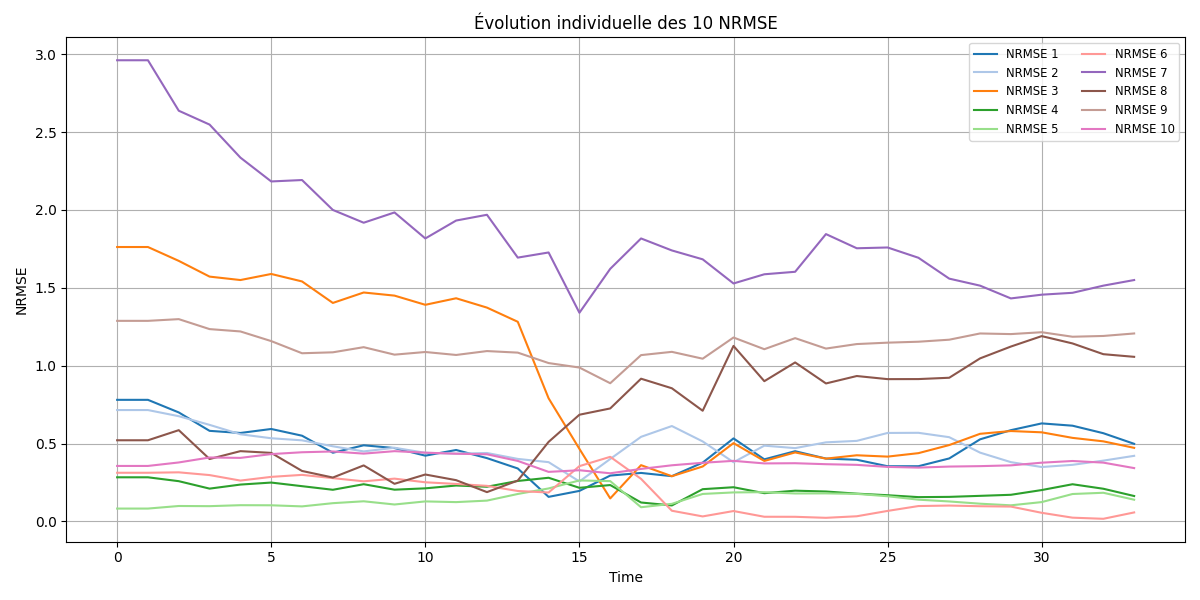
\includegraphics[width=0.8\textwidth]{images/UpdtC14_10NMRSE.png}
    \caption{Evolution of the NRMSEs over EnKF analysis phases}
    \label{fig:UpdtC14_10NMRSE}
\end{figure}

\textbf{4. More global interpolation}

The following explanations are based on the \autoref{fig:augmentedCoords}.
The minimum is found based on the blue cercles "coords\_seventh" interpolated points and averaged on the "avg\_seventh\_360" red point localisation. To try to have a more uniform field solution, we can average the parameters over a larger area, i.e., over 360 degrees instead of $360/7$ degrees. This allows to have a more global view of the parameters and to avoid local minima (green squares "coords\_7" average on the red cercles). But this can also lead to a solution that does not respect the periodicity of the pump, i.e., the solution is not 7 times the same pattern. So we can also average the parameters over 7 segments of $360/7$ degrees, which allows to have a more uniform field solution while respecting the periodicity of the pump (orange cruses "coords\_360" and purple cercles "avg\_7"). In this last case, the length of the coordinate of the observation points is 105 (5 variables, 3 PIV planes, and 7 segments of $360/7$ degrees) and the length of the observation vector is 315 (3 dimensions, 105 points).
%Pour cela j'ai commencé en moyennant 1/7 mais les paramètres étant locaux (non globaux), j'ai ensuite moyenné sur 360 degrés, ce qui permet de mieux prendre en compte les variations locales des paramètres. Cependant, nous pouvons converger vers une moyenne physique qui atteinds un minimum local mais qui ne respecte pas d'avoir 7 fois le même pattern. Cela permet à Fx d'être très différent de Fy mais aussi à la simulation de diverger avec des paramètres et vitesses erronéees. Pour palier ce problème, je compare la moyenne des patternes sur mes 7 segments de 360/7 degrés.

\begin{figure}[H]
    \centering
    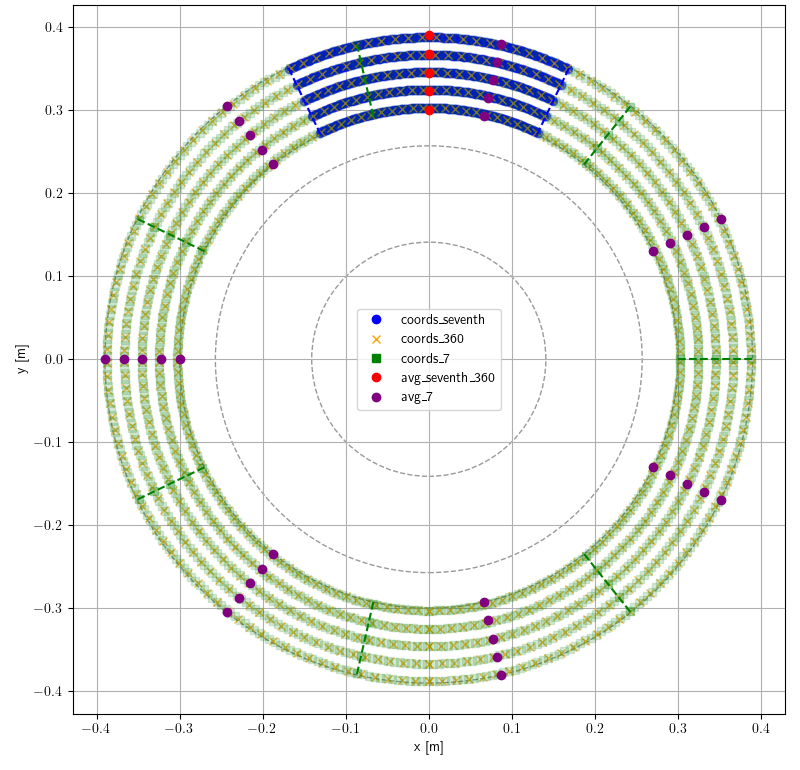
\includegraphics[width=0.8\textwidth]{images/numericalPump/coords.png}
    \caption{Illustration of the augmented coordinates for the interpolation of the field}
    \label{fig:augmentedCoords}
\end{figure}

\textbf{5.Inflation} The inflation strategy (explained in the \autoref{eqn:inflation}) is to use a more complex DA method, such as the EnKF with inflation, which allows to escape from local minima by adding noise to the ensemble members. This can help to explore the parameter space more effectively and find a better solution. But we didn't have this problem in our case so it hasn't been used.

\textbf{6.Pressure observation} Finaly, we can also add a pressure observation to the DA, which allows to take into account the pressure difference between the inlet and the outlet of the pump. This can help to improve the convergence of the solution and to have a more physical result. The pressure observation represents the difference of pressure between the inlet of the pipe and the outlet of the diffuser. The numerical coefficients are interpolating, respectively at (0,0,-0.35) and (0,0.390,0). Incertitude on p will be less than the measured one to take it better into account.
This implementation add one element on the observation vector.

%Sans inflation pour commencer. Si on converge vers une solution qui ne nous satisfait pas, on peut essayer d'ajouter... Cela permet de s'échaper d'un minimum local en ajoutant du bruit artificiellement. 

\begin{figure}[H]
    \centering
    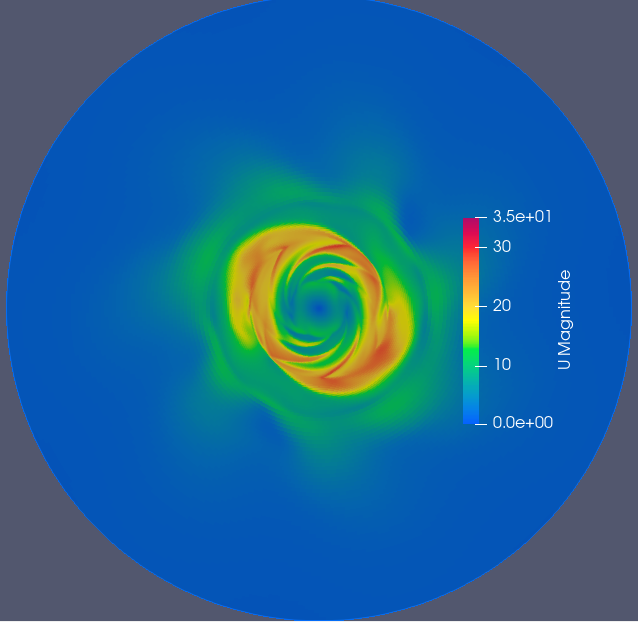
\includegraphics[width=0.5\textwidth]{images/numericalPump/assymetrie.png}
    \caption{Velocity field for Dx = 4e7 and Dy = 2e7}
    \label{fig:assymetry}
\end{figure}

After applying these strategies, the solution is still not satisfactory, as we can see in the \autoref{fig:UpdtC14_10NMRSE} where the NRMSEs remain high and the velocity field is still not physical and not converged.

\newpage
\section{Conclusion and outlook}

\textbf{Technical and human assessment}
% ///// Reprendre les objectifs définis à la fin de la section 2.1 //////

%Bilan technique et humain. Liez chaque aspect technique à un aspect humain. Ne traitez pas tout ce qui est technique d’un côté et tout ce qui relève de l’humain d’un autre. Réflexion personnelle sur les spécificités de l’entreprise, du secteur d’activité et du métier que vous avez découverts.

The first thing that I discovered during this internship is the laboratory environment, which is different from a company. The work is more focused on research, and there is a lot of freedom to explore new ideas and methods. The team is very collaborative and supportive, and I learned a lot from my colleagues. I also discovered the importance of communication and documentation in a research environment, as it is essential to share knowledge and results with others. There are still similaritys with a company, such as the social and environmental responsibility, that I presented in a first part.

After having done a state of art on the topics, we saw that the DA method is a good candidate to DNS or costly LES, for industrial applications, because it allows to have a good accuracy with a lower computational cost. I saw that an international expertise on application relies on this topic has been developed in the last few years on the laboratory. Numerical ingredients and usefull libraries were presented. The state of art was a good opportunity to learn more about the DA method and its applications. It was not too hard because most of information were already known by the laboratory. I also learned a lot about the IBM method and its applications, which is a good alternative to the traditional methods for the simulation of complex geometries.

Then, an explanation of the pump modeling, the pre-processing of the experimental data and the implementation of the IBM method in OpenFOAM were given. The redaction of this part helps me to structure my thoughts and to better understand the different steps of the pre-processing. I also learned a lot about the IBM method and its implementation in OpenFOAM, which was not easy at the beginning because I had to learn a lot about OpenFOAM and C++ programming. The implementation of the IBM method was a good opportunity to learn more about OpenFOAM and its functionalities.

Finally, we presented the first results of the numerical simulation and the first application of the DA method on the centrifugal pump case.
The results show that the IBM method as applied here does not give us a result consistent with physical observations and the DA does not allow us to improve this result. The solution is not converging and the velocity field is not physical, with a recirculation bubble in the diffuser. Several strategies were tested to try to improve the solution, but none of them allowed to obtain a satisfactory result.

I really enjoyed this internship beacause I learned a lot about all the topics that I love. That is why I decided to continue to work on this topic for my PhD thesis "Combining experimental and numerical techniques for the analysis of axial compressor internal flows using Data Assimilation" in the same laboratory.

\textbf{Outlook}

To continue this work, it would be interesting to try to change the IBM method (try the "interpolation method" for example) or to try an instationnary (URANS or LES) simulation to see if it can overcome these non-physical results.

The DA method is still not widely used in the industry, but it has a lot of potential for the future. The main challenge is to adapt the DA method to the specific needs of the industry, such as the use of complex geometries and the need for real-time applications. I discovered that DA can be long to implement and sometimes difficult to converge. At same time, EnKF needs a huge number of CPUs. Sometimes, I need to wait several days to launch a simulation. It would be interesting to try to reduce the computational cost of the DA method, by using more efficient algorithms or by using machine learning techniques, as presented in the state of art.
The IBM method is a good alternative to the traditional methods for the simulation of complex geometries, because it allows to have a good accuracy with a lower computational cost. An other challenge is to improve the accuracy of the IBM method.
%Outlook : Pb de la DA: plus rapide que LES mais toujours plus lent que RANS et le temps d'attente et de calcul sur supercalculateur (sur 4000 processeurs) est de l'orde de plusieurs jours. On peut donc se demander si la DA est vraiment utile dans ce cas. En effet, la DA est plus rapide que la LES mais pas que la RANS. Cependant, il faut prendre en compte le fait que la DA permet de réduire le temps de calcul de la simulation numérique en permettant d'optimiser les paramètres de l'IBM. De plus, la DA peut être utilisée pour d'autres cas d'étude où la LES est trop coûteuse.

\textbf{NOTES PERSO CI-DESSOUS}


Reduction of the pipe (with the research of the velocity inlet condition)

%Toujours mentionner les paramètres utilisés (dans le controlDict et le conesDict)

Problème de méthode et pas de miracle ave cette méthode IBM. Interpolation, instationnaire (avantage: on ne contraint plus avec MRF et donc plus facile de réconcilier solution numérique physique et mathématique)

Parler des coefficients de relaxation.

%Ouverture: méthode IBM interpolation, article non référencé.

%\cite{valeroEnhancedStateEstimation2025} -> ML turbulent channel flow Miguel

"Ouverture / idée": DA temps réel dans avion impossible pour encore longtemps.
Solution: Contrôle actif de la puissance en fonction des mesures de pression dans le compresseur:
f(obs) -> controle de la puissance
Pour ça, se ref au sujet de thèse de Tarane
obs pression --> modèle de reconstruction du champ de vitesse --> modèle de reconaissance de patternes de décrochage --> contrôle de la puissance
Peut-être faire deux filtres de Kalman imbriqués ? hyperparamètres type fenetre observation, variance initiale, ...


Voir "TD -> Done et "TDSave -> Done" pour voir tt ce que j'ai fais

The random variations are random but with a reproducibility seed (sed) that allows to have the same result each time the simulation is launched.


The theorical average radial speed at the input of the diffuser is equal to \[\frac{Q_{dif_{in}}}{S_{dif_{in}}} = \frac{Q_{pump_{in}}}{2\pi R_{3} h_{dif}} = 3.65m.s^{-1}\]
With $Q_{pump_{in}} = Q_{dif_{in}}$ because the mass flow rate is constant and the flow is incompressible.// -> No need ??

\begin{figure}[H]
    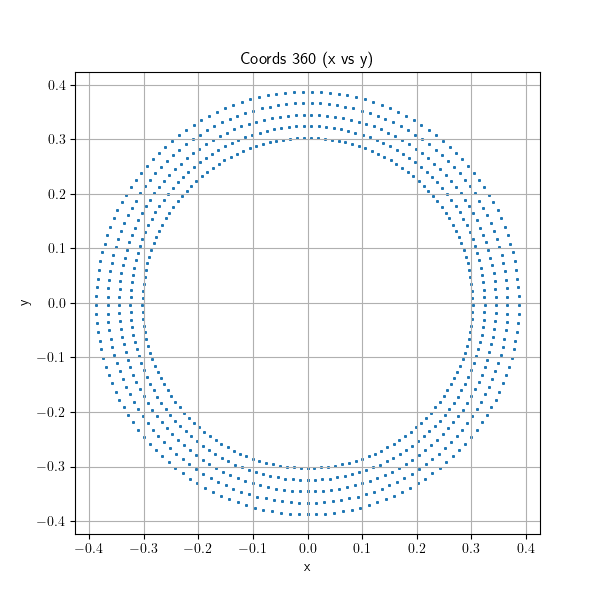
\includegraphics[width=0.4\textwidth]{images/coords360.png}
    \caption{Interpolation points over 360 degrees}
    \label{coords360}
\end{figure}

Methodo (forcage continue (vs interpolation ?)) -> avantages

%////Annexe des opérateurs grad, div, nabla, rot, laplacien, laplacien vectoriel, etc...////

The EnKF method will be used to assimilate data from the flow at the observation points and to update the forcing term until it converges to the optimal value. These high-fidelity data are obtained from an experiment explained in the next \autoref{sec:Experimental_data_and_pre-processing}.


%En combien de temps l'information de pression remonte-t-elle dans le diffuser ? -->> "directement"
%144 coeurs: 54it/min
%300-> 336 coeurs: 100it/min (+- 20\%)

%Limitations IBM à améliorer avec DA

Graçe aux données xp (mentionné partie 2.1.2, on peut faire de la DA)

Check consistance U, u, P, p, gras, italique,... dans les équations

Comparer les 2-3 résultats: (avant DA, déjà fait section précédente), après simple et "complex" DA

Supposons 1000 itération en moyenne entre chaque phase d'analyse, et 300 phases d'analyse, cela nous fait 300 000 itérations à simuler, soit 93h, sur env. 2800 coeurs, soit 264kh.processeur de calcul.

Verif que j'ai mis ttes les images présentes dans le dossier "images"

%Intro simple - globale

% Essayer d'améliorer le rendu de l'image ci-dessous en mettant la pompe en transparence

%L'expérience montre un ordre de grandeur de centaines d'itération entre les phases d'analyse, mais cela dépend beaucoup du cas.
%Il en est de même pour le nombre de phases d'analyse.